%%%%%%%%%%%%%%%%%%%%%%%%%%%%%%%%%%%%%%%%%
% Short Sectioned Assignment
% LaTeX Template
% Version 1.0 (5/5/12)
%
% This template has been downloaded from:
% http://www.LaTeXTemplates.com
%
% Original author:
% Frits Wenneker (http://www.howtotex.com)
%
% License:
% CC BY-NC-SA 3.0 (http://creativecommons.org/licenses/by-nc-sa/3.0/)
%
%%%%%%%%%%%%%%%%%%%%%%%%%%%%%%%%%%%%%%%%%

%----------------------------------------------------------------------------------------
% PACKAGES AND OTHER DOCUMENT CONFIGURATIONS
%----------------------------------------------------------------------------------------

\documentclass[paper=a4, fontsize=11pt,numbers=endperiod]{scrartcl} % A4 paper and 11pt font size

\usepackage[T1]{fontenc} % Use 8-bit encoding that has 256 glyphs
%\usepackage{fourier} % Use the Adobe Utopia font for the document - comment this line today return to the LaTeX default
\usepackage[english]{babel} % English language/hyphenation
\usepackage{amsmath,amsfonts,amsthm} % Math packages

\usepackage[utf8]{inputenc} % Needed to support swedish "åäö" chars
\usepackage{titling} % Used to re-style maketitle

\usepackage{lipsum} % Used for inserting dummy 'Lorem ipsum' text into the template

\usepackage{sectsty} % Allows customizing section commands
\allsectionsfont{\normalfont} % Make all sections the default font

% Local packages:
\usepackage{enumerate}
\usepackage[usenames,dvipsnames]{color}
\usepackage{tabularx}
\usepackage{fancyvrb}
\DefineShortVerb{\|}
\usepackage{hyperref}
\usepackage{url}
\usepackage[parfill]{parskip}   % Sets newlines between paragraphs
\usepackage{algorithm2e} % Used for Pseudocode
\providecommand{\abs}[1]{\lvert#1\rvert} % \abs{x+y} produces |x+y|
\usepackage{graphicx}
\DeclareGraphicsExtensions{.png,.jpg}
\usepackage{sectsty}
\usepackage{fancyhdr} % Custom headers and footers
\pagestyle{fancyplain} % Makes all pages in the document conform to the custom headers and footers

% Header with additional info
% \fancyhead[L]{\small{Gustaf Lindstedt - \href{mailto:glindste@kth.se}{\color{RoyalBlue}\nolinkurl{glindste@kth.se}} - 910301\\Martin Runelöv - \href{mailto:mrunelov@kth.se}{\color{RoyalBlue}\nolinkurl{mrunelov@kth.se}} - 900330-5738}}
% Simple header
\fancyhead[L]{\small{Gustaf Lindstedt\\Martin Runelöv}} % 


\fancyfoot[L]{} % Empty left footer
\fancyfoot[C]{} % Empty center footer
\fancyfoot[R]{\thepage} % Page numbering for right footer
\renewcommand{\headrulewidth}{0pt} % Remove header underlines
\renewcommand{\footrulewidth}{0pt} % Remove footer underlines
\setlength{\headheight}{23.0pt} % Customize the height of the header
\fancyhfoffset[L]{10mm}% slightly less than 0.25in

\numberwithin{equation}{section} % Number equations within sections (i.e. 1.1, 1.2, 2.1, 2.2 instead of 1, 2, 3, 4)
\numberwithin{figure}{section} % Number figures within sections (i.e. 1.1, 1.2, 2.1, 2.2 instead of 1, 2, 3, 4)
\numberwithin{table}{section} % Number tables within sections (i.e. 1.1, 1.2, 2.1, 2.2 instead of 1, 2, 3, 4)


\allsectionsfont{\bfseries}

\setlength\parindent{0pt} % Removes all indentation from paragraphs - comment this line for an assignment with lots of text


\posttitle{\par\end{center}} % Remove space between author and title
%----------------------------------------------------------------------------------------
% TITLE SECTION
%----------------------------------------------------------------------------------------

\title{ 
\huge Project 2 - Euclidean TSP \\ % The assignment title
\vspace{10pt}
\normalfont \normalsize 
\textsc{DD2440 - Advanced algorithms } \\ [25pt] % 
}

\author{Gustaf Lindstedt \\ glindste@kth.se \\ 910301-2135 \and Martin Runelöv \\ mrunelov@kth.se \\ 900330-5738}

\date{\vspace{8pt}\normalsize\today} % Today's date or a custom date

\begin{document}

\maketitle % Print the title


%-------------------------------------------------------------------------------
% SECTION 1
%-------------------------------------------------------------------------------
\hspace{0pt}\\
\section*{Statement of collaboration}
All of the research was done together, and the report was written together.
Gustaf implemented the initial 2-opt, and Martin implementented the initial 2.5-opt.
Gustaf did the initial satellite lists and neighbour list initialization. Gustaf reworked 2-opt to work with satellite lists.
Martin reworked 2.5-opt to work with satellite lists, and reworked Nearest Neighbour and 2.5-opt to work with with the neighbour lists.
Gustaf implemented the initial 3-opt algorithm.

\section{Introduction}

% heh orkade inte ha ett intro direkt med underrubrik.
This project was done as part of the course \emph{Advanced Algorithms} at the Royal Instityte of Technology, KTH.

\subsection{Problem}

The traveling salesman problem (TSP) is famous in both theoretical computer science and in operations research. It asks the following question: 

\begin{center}
    \emph{Given a list of cities and the distance between each pair of cities, what is the shortest possible route that visits each city exactly once and returns to the origin city?}
\end{center}

This combinatorial problem is NP-hard and therefore requires heuristics and approximation algorithms to be approximated within reasonable time for larger instances.

Our problem is a special case of TSP which consists of finding such a tour in Euclidean space. This means that a distance from city A to city B is equal to the distance from B to A, and that the triangle inequality holds. There is no designated origin city, meaning that it can be arbitrarily chosen.
However, the problem is still NP-hard.

%-------------------------------------------------------------------------------
% SECTION 2
%-------------------------------------------------------------------------------
\section{Algorithms}

\subsection{Nearest neighbour}
The nearest neighbour (NN) algorithm is a greedy strategy. It is very unlikely that it will return the optimal solution, but it find an approximated solution in reasonable time.
The heuristic works as follows: 
Every node is marked as visited once it has been used so the tour doesn't revisit any nodes.
Pick a node's nearest available neighbour as the next node in the tour.

Once all nodes have been visited the tour is complete.

\subsection{Local optimization algorithms}
When a tour has been calculated, we can apply local optimization techniques by examining parts of the tour. We are not guaranteed to find optimal solutions by iterating these indefinitely since they can get stuck in local minimums, but used correctly they can provide significant improvements.

\subsubsection{2-opt}
2-opt is a local search optimization in which pairs of edges are selected andevaluated if they would provide a better tour if they swapped nodes.
Take two edges A-B and C-D for example.
If the sum of the two edges A-C and B-D is smaller than the initial sum, then the edges should be swapped.
At this point the subpath from B to C should be reversed, so that it is traversed from C to B instead, in order to retain the rest of the tour configuration.

\begin{center}
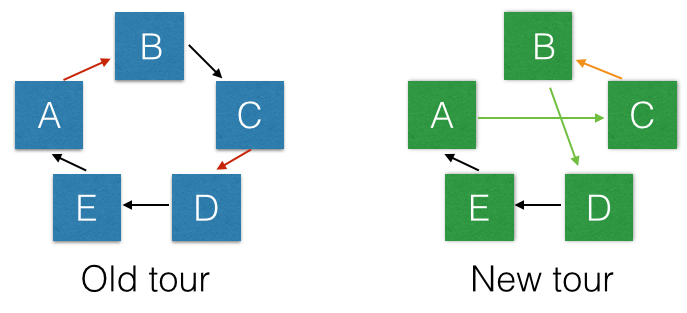
\includegraphics[scale=0.4]{2opt}
\end{center}

\subsubsection{2.5-opt}
2.5-opt, also known as 2h-opt, works as follows:

Pick one city B. B is currently between cities A and C. Try to move B to between any other two cities D and E such that the total distances becomes shorter. With $d$ being the distance function for two cities, we are looking for cities A-E such that the following is true:
\[
    \underbrace{d(A,B) + d(B,C) + d(D,E)}_\text{Old distances}\; > \;\underbrace{d(A,C) + d(D,B) + d(B,E)}_\text{New distances}
\]

The below image illustrates the concept:

\begin{center}
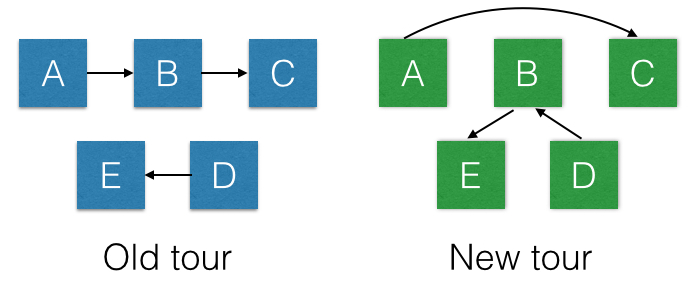
\includegraphics[scale=0.4]{25opt}
\end{center}

\subsection{3-opt}
3-opt works similarly to two opt, the difference being that three edges are chosen for swapping instead of two.
Given three edges A-B, C-D and E-F there are 8 unique configurations involving the nodes, of which one is the original configuration.
Three configurations are covered by the 2-opt algorithm, since they only modify two of the three edges.
This leaves four different configurations involving modification of all three edges.
The difference in distance is calculated for each configuration and compared to the others.
If a configuration leads to a better distance than the original and all the other configuration the swap is performed.

<pic>
    

%----------------------------------------------------------------------------------------
% SECTION 3
%----------------------------------------------------------------------------------------
\section{Implementation}
The program was implemented in the C programming language.

The nearest neighbour algorithm was used to calculate a first naive solution upon which local search optimizations could be made.
Most of the loops over nodes start with a random node, since it yielded improved results.
\subsection{Neighbour lists}
Lists of every nodes closest neighbours were calculated at the start in order to speed up certain algorithms.
The Nearest Neighbour algorithm took advantage of this, as did 2.5-opt. When using neighbour lists, only a small combination of cities is checked, but they often provide good estimates of good paths between cities and the trade-off is often worth it in practice.

\subsection{Satellite lists}
In order to effectively perform the local optimizations a specialized data structure is required.
In particular, we need to optimize operations such as reversing a subtour, and moving a city.
To move a city, we need a structure that has tour positions that are independent from other parts of the tour.
This can be achieved with a doubly linked list since it allows us to easily move individual cities.

However, to optimize reversal of a subtour we need something called a \emph{satellite lists}.\cite{satellite}
A satellite list uses two reference values for every node, called satellites.
They point to satellites of other nodes, one pointing to a satellite which belongs to the next node and the other to a satellite belonging to the previous node.
The satellites only point to other satellites pointing in the same direction as them.
This creates two ``flows'' in the satellite list, which are independent from each other but linked in that they are each others reverse.

A satellite list can easliy be implemented using a doubly sized array.
Each index corresponds to a satellite, and satellites are grouped in pairs by node.
The value of an index is the index of the satellite that the current satellite points to.

This structure provides the ability to reverse a subtour in O(1) time.
One simply relink the satellites so that the ``forward'' flow links in to the ``reverse'' flow of the subsection, and then link back to the forward flow at the end.
This operation is mirrored for the complement satellites.


% OBS OBS OBS
% OBS OBS OBS
% We might need to explain the operations in the table (bitshift, XOR etc.)
% , and we should think about where to place the image. My first thought is to place
% it at the bottom of the section.
% OBS OBS OBS
% OBS OBS OBS
\begin{center}
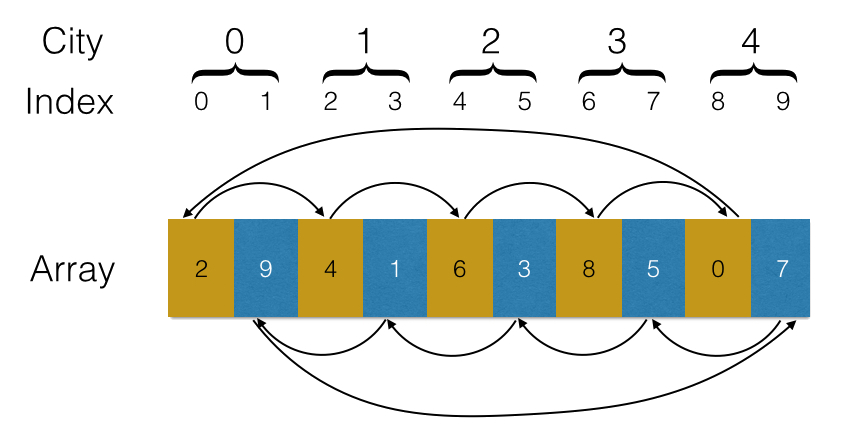
\includegraphics[scale=0.3]{satellite}
\end{center}

Using this structure, we can infer the following:\\
\begin{table}[h]
  \centering
  \begin{tabular}{|c|c|}
    \hline
    Index of a satellite & $i$ \\ \hline
    Node of a satellite & $i>>1$ \\ \hline
    The complement satellite & $i$\^{}1 \\ \hline
  \end{tabular}
\end{table}


Note that the above image is a depiction of a possible (starting) configuration. The ''satellites'' (indexes 0-9) can point to any other index in the array.

\subsection{Opts}
All k-opt optimizations had the possibility to randomize their starting point.

The 2-opt algorithm have a complexity of O($n^2$), since we try every possible edge pair.

2.5-opt was implemented using neighbour lists.
This reduced its time complexity from O($n^2$) to O($n\times nl$) where $nl$ is the length of a neighbour list.

3-opt is O($n^3$) since it iterates over edge triples.
However, the implementation in our best version had an O($n^2$) algorithm due to a bug.
The bug caused it to try one edge as the third one, which was the one directly following the second edge.
When the bug was fixed the result worsened, probably due to the increased complexity.

\subsection{Introducing randomness}
A significant problem with local optimization techiques is the posibility of reaching a local minimum which is suboptimal.
One solution to this is to ``destroy'' the local minimum by swapping a few random edges and performing the local search again.
This can help the solution to break away from the local minimum and achieve a better result.
This cycle of introducing randomness and performing local optimization can be repeated indefinitely providing that the best solution is always saved.

%------------------------------------------------------------------------------
%   SECTION 4
%-------------------------------------------------------------------------------

\section{Results}

Every algorithm led to improvements, and 

\begin{table}[h]
  \centering
    \begin{tabular}{|c|c|c|c|c|}
    \hline
    \textbf{Algorithm} & \textbf{Best Score} \\ \hline
    Nearest Neighbour & 3 \\ \hline
    2-opt & 19 \\ \hline
    2.5-opt & 25 \\ \hline
    Random swaps & 33 \\ \hline
    3-opt & 36\textsuperscript{*} \\ \hline
    \end{tabular}
    \caption{Kattis result table. All rows includes all features of the ones above}
    \hspace{10pt}
  \end{table}

\textsuperscript{*}Kattis ID for the best submission: \href{https://kth.kattis.scrool.se/submission?id=469874}{469874}

% TODO: skriva om storlek på neighbour lists!!! 30-40 är bäst för största indatan!

Experiments showed that small neighbour lists gave the best results. Since they need to be sorted they can be expensive to create, and there is therefore an equilibrium to be found where the trade-off is optimal. We didn't try different sizes extensively, but our tests showed that neighbour lists of length 20-40 gave us the best trade-off.




\section{Discussion}

% Nåt generellt om projektet kanske. 

The drawback of using a satellite list is that we can't know the direction of a city's satellites relative to another city without traversing the subtour between them.
This means that two randomly chosen nodes can't be used directly when reversing a subtour since we won't know which satellites should be remapped and to where in order to retain flow integrity.
This caused problems with neighbour lists since this means that we can't use them where swapping is needed without introducing the overhead of traversing the entire tour to find their orientation.

However, both Nearest Neighbour and 2.5-opt was able to utilize neighbour lists since there is no subtour reversal involved in these algorithms.

% Nåt om satellite antar jag. Dom är lite dryga.
All concepts and algorithms used are relatively easy to understand, but they became harder to implement with satellite lists.
The satellite lists required us to think carefully when changing the tour.


\subsection{Future work}

Given more time we would have liked to implement a k-level tree, or a k-level satellite tree.
A k-level tree enables O($\log{n}$) traversal time, which would have allowed us to theoretically speed up both 2-opt and 3-opt with the usage of neighbour lists.

Using k-level trees we could have used stem-and-cycle ejection chain algorithms, which are said to be the best known local search methods for TSP.\cite{stem-cycle}

There are also some interesting Ant Colony Optimization (ACO) algorithms that shows promise. These algorithms are a fun concept, and given more time we would have investigated this approach further. \cite{ACO}
% OBS: ACO-källan gäller probabilistisk TSP (annan sorts TSP), men källan gäller egentligen bara konceptet.

% Avsluta med något om hur nöjda vi är?



%----------------------------------------------------------------------------------------
% REFERENCES
%----------------------------------------------------------------------------------------
\newpage
\begin{thebibliography}{9}

% TODO TODO TODO TODO TODO TODO TODO  TODO TODO TODO TODO  TODO TODO TODO TODO 
% INSERT GODDAMN DATES!
\bibitem{algnotes} Notes for the course advanced algorithms - \url{http://www.nada.kth.se/~johanh/algnotes.pdf} <insert date here!>
 
\bibitem{satellite} Osterman, Colin, et al. \emph{The satellite list and new data structures for symmetric traveling salesman problems.} (2004).

\bibitem{stem-cycle} Harabor, Daniel, and Philip Kilby. "Informed Heuristics for Guiding Stem-and-Cycle Ejection Chains." arXiv preprint arXiv:1103.3904 (2011).

\bibitem{ACO} Bianchi, Leonora, Luca Maria Gambardella, and Marco Dorigo. "An ant colony optimization approach to the probabilistic traveling salesman problem." Parallel Problem Solving from Nature—PPSN VII. Springer Berlin Heidelberg, 2002. 883-892.
\end{thebibliography}

\end{document}
